\documentclass[12pt]{article}
\usepackage[top=1in,left=1in, right = 1in, footskip=1in]{geometry}

\usepackage{graphicx}
%\usepackage{adjustbox}

\newcommand{\eref}[1]{(\ref{eq:#1})}
\newcommand{\fref}[1]{Fig.~\ref{fig:#1}}
\newcommand{\Fref}[1]{Fig.~\ref{fig:#1}}
\newcommand{\sref}[1]{Sec.~\ref{#1}}
\newcommand{\frange}[2]{Fig.~\ref{fig:#1}--\ref{fig:#2}}
\newcommand{\tref}[1]{Table~\ref{tab:#1}}
\newcommand{\tlab}[1]{\label{tab:#1}}
\newcommand{\seminar}{SE\mbox{$^m$}I\mbox{$^n$}R}

\usepackage{amsthm}
\usepackage{amsmath}
\usepackage{amssymb}
\usepackage{amsfonts}

%\usepackage{lineno}
%\linenumbers

\usepackage[pdfencoding=auto, psdextra]{hyperref}

\usepackage{natbib}
\bibliographystyle{chicago}
\date{\today}

\usepackage{xspace}
\newcommand*{\ie}{i.e.\@\xspace}

\usepackage{color}

\newcommand{\Rx}[1]{\ensuremath{{\mathcal R}_{#1}}} 
\newcommand{\Ro}{\Rx{0}}
\newcommand{\RR}{\ensuremath{{\mathcal R}}}
\newcommand{\Rhat}{\ensuremath{{\hat\RR}}}
\newcommand{\tsub}[2]{#1_{{\textrm{\tiny #2}}}}

\newcommand{\comment}[3]{\textcolor{#1}{\textbf{[#2: }\textsl{#3}\textbf{]}}}

%% \newcommand{\rev}[1]{\comment{red}{REV}{#1}}
\newcommand{\rev}[1]{}

\newcommand{\swp}[1]{\comment{magenta}{SWP}{#1}}
\newcommand{\new}[1]{\textcolor{blue}{#1}}

\begin{document}

\begin{flushleft}{
	\Large
	\textbf\newline{
		Evaluating uncertainties associated with early estimates of the basic reproduction number during the novel coronavirus (2019-nCoV) outbreak
	}
}
\newline
\\
Sang Woo Park\textsuperscript{1}
Jonathan Dushoff\textsuperscript{2,3}
\\

\bigskip
\textbf{1} Department of Ecology and Evolutionary Biology, Princeton University, Princeton, New Jersey, USA
\\
\textbf{2} Department of Biology, McMaster University, Hamilton, Ontario, Canada
\\
\textbf{3} Michael G. DeGroote Institute for Infectious Disease Research, McMaster University, Hamilton, Ontario, Canada
\\
\bigskip

% *swp2@princeton.edu
\end{flushleft}

\section*{Abstract}

\pagebreak

\section{Introduction}

Since the end of December 2019, a novel coronavirus (2019-nCoV) continues to
spread in China and in other parts of the world.
As of January 27th, 2020, the World Health Organization has
confirmed 2798 cases, including 37 confirmed cases in 11 different
countries, outside China \citep{who27report}.
Although the virus is suspected to have originated
from animal reservoirs, a recent case from Viet Nam
demonstrated its ability to transmit between
humans \citep{who26report},
posing a greater threat for a wider spread.

Many researchers have been rushing to publish their 
analysis of the outbreak \citep{imaincov, riouncov,readncov,zhaoncov,majumderncov,liuncov} 
and, in particular, their
estimates of the basic 
reproductive number $\mathcal R_0$ (i.e., the 
average number of secondary cases generated 
by a primary case in a fully susceptible population).
The basic reproductive number is of particular interest 
because it allows prediction about the final size of an epidemic.
While their efforts are valuable, their analyses rely on several
assumptions that could immediately affect their estimates of $\mathcal R_0$ and
the associated uncertainties.

Here, we present a simple framework for evaluating uncertainties 
associated with parameter estimates
across a wide range of models.
Our results indicate that most published estimates of $\mathcal R_0$
are likely to be overly confident. 
We also lay down several principles that needs to be taken into
consideration.

\section{Methods and results}

Early in an outbreak, $\mathcal R_0$ cannot be estimated directly.
Instead, estimates of $\mathcal R_0$ are often inferred from
the exponential growth rate $r$, which can be estimated reliably from incidence data.
Given estimates of the exponential growth rate $r$ and the distribution $g(\tau)$ of
generation intervals (i.e., the time between when a person become 
infected and that person infects another person), the basic reproduction
number can be estimated via the Euler-Lotka equation:
\begin{equation}
1/\mathcal R_0 = \int \exp(-r\tau) g(\tau) d\tau.
\end{equation}
In other words, estimates of $\mathcal R_0$
will depend on the assumptions about the
exponential growth rate $r$ and the shape of generation-interval distribution $g(\tau)$.

\begin{figure}[t]
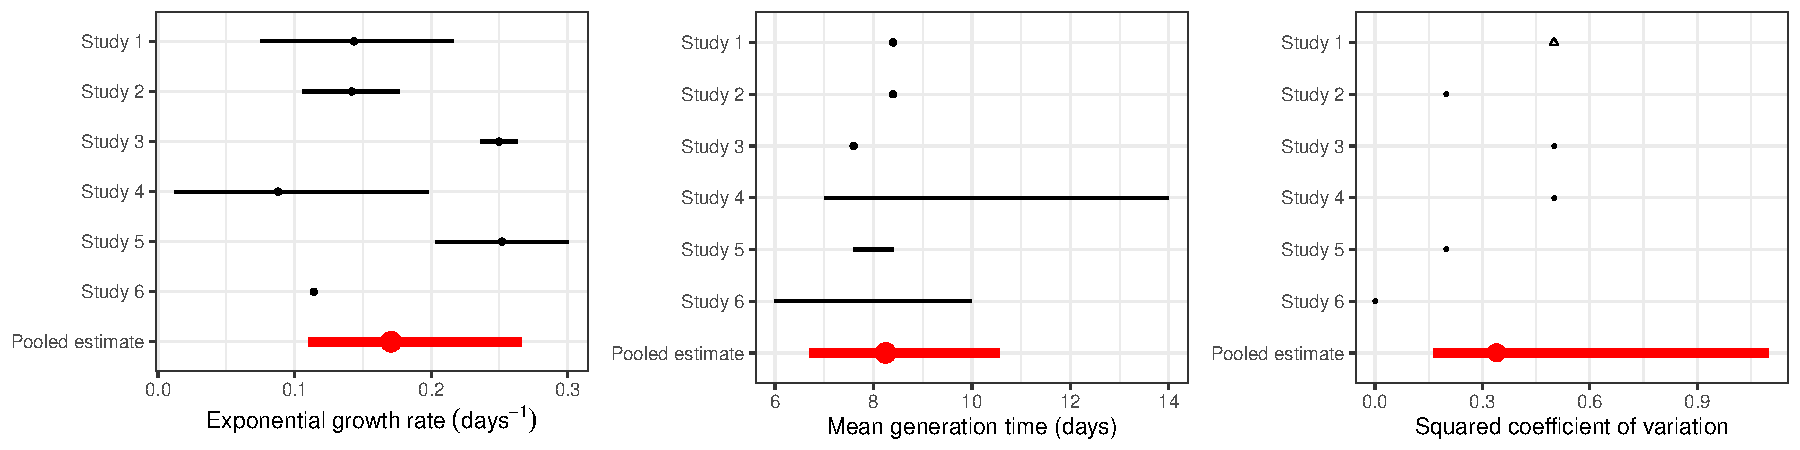
\includegraphics[width=\textwidth]{compare_assumption.pdf}
\caption{
Early estimates of $\mathcal R_0$ and associated assumptions about $r$ and $g(\tau)$.
}
\end{figure}

We use the gamma approximation framework to first characterize the
amount of uncertainty present in the underlying parameters and then 
to assess the 
degree to which these uncertainties
affect the estimate of $\mathcal R_0$.
Assuming that generation intervals follow a gamma distribution 
with the mean $\bar G$ and the squared coefficient of variation $\kappa$, 
we have
\begin{equation}
\mathcal R_0 = \left(1 + \kappa r \bar{G}\right)^{1/\kappa}.
\label{eq:gamma}
\end{equation}
This equation demonstrates that a generation-interval distribution
that assumes a larger mean (higher $\bar{G}$) or is less variable (lower $\kappa$)
will give a higher estimate of $\mathcal R_0$ for the same value of $r$.

First, we gather information on estimates of $\mathcal R_0$ and their
assumptions about the underlying generation-interval distributions from preprint servers (e.g., bioRxiv, medRxiv, and SSRN).
For each study, we model $\mathcal R_0$, $\bar G$, and $\kappa$ with an appropriate probability distribution (either uniform or gamma) that roughly matches the estimated or assumed values and uncertainty ranges.
For example, \cite{imaincov} estimated $\mathcal R_0 = 2.6$ (95\% CI: 1.5--3.5);
we model this parameter as a gamma distribution with mean of 2.6 and a shape parameter of 28, which has a 95.2\% probability of containing a value between 1.5 and 3.5.
Then, we draw 100,000 random samples from these distributions and calculate the exponential growth rate $r$ via the inverse of \eref{gamma}:
\begin{equation}
r = \frac{\mathcal R_0^\kappa - 1}{\kappa \bar{G}}
\end{equation}

To define ranges of appropriate uncertainties for each parameter ($r$, $\bar G$, and $\kappa$),
we use a Bayesian multilevel modeling approach by assuming that all \emph{observed} (i.e., estimated or assumed) parameter values come from the same distribution:
\begin{equation}
\begin{aligned}
r_i &\sim \mathrm{Gamma}(\mathrm{mean}=\mu_r, \mathrm{shape}=\alpha_r),\\
\bar{G}_i &\sim \mathrm{Gamma}(\mathrm{mean}=\mu_G, \mathrm{shape}=\alpha_G),\\
\kappa_i &\sim \mathrm{Exponential}(\mathrm{mean}=\mu_\kappa),\\
(\mu_r, \alpha_r, \mu_G, \alpha_G, \mu_\kappa) &\sim \mathrm{Gamma}(\mathrm{shape}=0.1, \mathrm{rate}=0.1),
\end{aligned}
\end{equation}
where $i$ represents the index across 6 studies that we consider.
We use an exponential distribution to model $\kappa_i$ to account for the fact that the IDEA model, which \cite{majumderncov} uses, assumes that the generation-interval distribution is fixed ($\kappa = 0$).
Hyperparameters $\mu_r$, $\alpha_r$, $\mu_G$, $\alpha_G$, and $\mu_\kappa$ are estimated with a Markov Chain Monte Carlo (MCMC) by drawing a random set for $r_i$, $\bar{G}_i$, and $\kappa_i$ at each MCMC step from the 100,000 samples that we calculated previously.
We run 4 parallel chains that consist of 100,000 burnin steps and 100,000 sampling steps.
Posterior samples are thinned every 200 steps.
Convergence is assessed by ensuring that the Gelman-Rubin statistic is below 1.01 for all hyperparameters \citep{gelman1992inference}.





\pagebreak

\bibliography{wuhan}

\end{document}
